% ---------------------------------------------------------------------------------------------
% Simulation check of the theory. Code: experiments/theory_check.py. Results: results/theory_check.json.
% Figures: figures/fig_sim_real.{pdf,png}, figures/fig_sim_rho.{pdf,png}.
% ---------------------------------------------------------------------------------------------
\section{Checking the theory by simulation}\label{sec:simulation}

Section~\ref{sec:theory} gives three predictions of the efficiency $\mathrm{Eff}_t=\mathrm{MSE}_{\rm SRS}/\mathrm{MSE}_{\rm PATTERN}$
of a comparison estimand $t$, in decreasing order of generality and increasing order of
simplicity:
\begin{itemize}
\item[LIN] the exact linearised design effect of the allocation actually used,
$N^2(1/L-1/N)S^2_t/V_t(n)$ with $V_t$ from \eqref{eq:linvar}; it is exact up to the linearisation
of Proposition~\ref{prop:validity} and includes the compromise between targets, the proxy-based
allocation, the minimum of 10 labels per stratum and the finite-population corrections;
\item[OWN] the own-target Neyman efficiency \eqref{eq:deff-general} on the pattern strata, which
removes the compromise and the proxy but keeps the actual strata;
\item[FORM] the closed form of Corollary~\ref{prop:deff}, \eqref{eq:deff-tpr} and
\eqref{eq:deff-err}, which assumes strata that separate the pair's agreements from its
disagreements, and its small-target version $1/\rho$.
\end{itemize}
All three are computed from the full pool, using the labels only to evaluate the formulas, and are
compared with Monte Carlo efficiencies. Everything in this section is produced by
\texttt{experiments/theory\_check.py} and stored in \texttt{results/theory\_check.json}.

\subsection{Real pools}\label{sec:sim-real}

We re-ran the SRS and PATTERN arms of the main study (Section~\ref{sec:empirical}) on the 11 cached
pools, at the same budgets, with $R=200$ replications and the same random seeds; the GROUP and ORACLE
samples are drawn as well, so that the random stream is identical. The resulting median efficiencies
coincide with those in \texttt{results/label\_efficiency.json} for all 35 pool--budget
combinations, so the per-target efficiencies below are those underlying the main results. A
target is compared when its influence values are not identically zero and its design variance is
positive. This removes the 45 targets of the 15 pairs of models with identical predictions in
Law school, a further six targets in that pool, and all targets of Law school at $L=2000$, where the
strata that carry the comparisons are fully enumerated and both the observed and the predicted
efficiency are infinite (the json reports $4\times10^{23}$). That leaves 3519 target--budget pairs.

\begin{table}[t]
\centering
\caption{Real pools: predicted and observed efficiency of PATTERN relative to SRS (medians over the
108 comparison estimands; $L=500$, $L=250$ for Spambase). $\rho_{\rm any}$: share of the pool on
which not all nine models agree; $\rho$: median pairwise disagreement rate. Obs: Monte Carlo
($R=200$; identical to \texttt{results/label\_efficiency.json}). LIN, OWN, FORM: predictions defined
in the text. Last two columns: per-target ratio Obs/LIN, median and 10\%--90\% range, and the
correlation of $\log$ Obs and $\log$ LIN across targets. Source: \texttt{results/theory\_check.json}.}
\label{tab:sim-real}
\small
\begin{tabular}{lrrrrrrrrll}
\toprule
Pool & $N$ & $\rho_{\rm any}$ & $\rho$ & Obs & LIN & OWN & FORM & $1/\rho$ & Obs/LIN & corr\\
\midrule
Adult-sex & 19537 & 0.51 & 0.069 & 4.08 & 3.97 & 5.43 & 13.22 & 14.5 & 1.03 (0.83, 1.27) & 0.95\\
Adult-race & 19537 & 0.51 & 0.070 & 6.02 & 6.68 & 7.47 & 18.71 & 14.2 & 0.98 (0.77, 1.20) & 0.98\\
Bank & 18085 & 0.18 & 0.053 & 7.87 & 7.17 & 9.08 & 22.47 & 18.8 & 1.02 (0.83, 1.25) & 0.96\\
Credit card & 12000 & 0.56 & 0.055 & 3.79 & 3.88 & 4.48 & 12.96 & 18.3 & 0.99 (0.84, 1.18) & 0.97\\
Law school & 8320 & 0.19 & 0.001 & 15.33 & 13.79 & 25.74 & 3.54 & 924 & 1.06 (0.96, 1.22) & 1.00\\
MAGIC & 7608 & 0.40 & 0.166 & 2.76 & 2.83 & 3.31 & 5.68 & 6.0 & 0.96 (0.78, 1.16) & 0.82\\
EEG & 5992 & 0.73 & 0.329 & 1.83 & 1.75 & 2.24 & 3.19 & 3.0 & 1.03 (0.88, 1.27) & 0.85\\
Phoneme & 2162 & 0.39 & 0.162 & 3.60 & 3.61 & 2.91 & 5.53 & 6.2 & 1.00 (0.84, 1.19) & 0.81\\
Spambase & 1841 & 0.32 & 0.086 & 5.55 & 5.63 & 5.13 & 12.02 & 11.6 & 1.00 (0.85, 1.24) & 0.92\\
Churn & 2000 & 0.19 & 0.084 & 32.36 & 32.15 & 5.95 & 11.29 & 11.9 & 1.02 (0.89, 1.21) & 1.00\\
Electricity & 12000 & 0.34 & 0.128 & 2.84 & 2.93 & 3.34 & 6.69 & 7.8 & 0.96 (0.82, 1.18) & 0.61\\
\bottomrule
\end{tabular}
\end{table}

\begin{figure}[t]
\centering
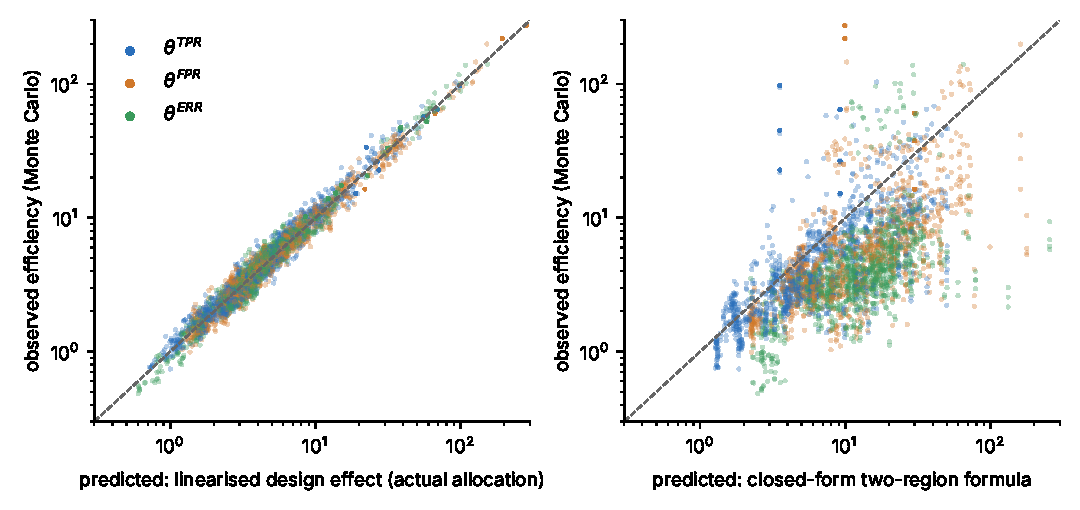
\includegraphics[width=\textwidth]{figures/fig_sim_real.pdf}
\caption{Real pools, all budgets: observed efficiency of PATTERN relative to SRS for each of the
3519 compared target--budget pairs against the linearised prediction LIN (left) and the closed-form
two-region formula FORM (right). Dashed: equality. Source: \texttt{results/theory\_check.json}.}
\label{fig:sim-real}
\end{figure}

\paragraph{The linearised design effect is accurate.} Over the 3519 pairs the ratio of observed to
predicted efficiency has median 0.998 and 10\%--90\% range 0.83--1.22; 77\% of the ratios are within
20\% and 99\% within a factor 1.5, and the correlation of the logarithms is 0.988
(Figure~\ref{fig:sim-real}, left). The spread is what Monte Carlo error alone produces: each MSE is
an average of 200 squared errors, with a relative standard error of about $\sqrt{2/200}=0.10$ for
approximately normal errors, so the ratio of two independent MSEs has a relative standard error of
about 0.14 and a 10\%--90\% range of roughly 0.84--1.20. The medians per pool and budget agree as
well: the ratio of the observed median efficiency to the median LIN prediction lies between 0.88 and
1.20 for the 34 pool--budget combinations, and for each type of estimand separately the median of
these ratios is 0.99 (TPR), 0.98 (FPR) and 1.00 (error). The agreement includes the cases with very
large gains: for Churn at $L=500$ the observed efficiency of 32.4 (predicted 32.2) arises because
the disagreement strata are fully enumerated, which only the finite-population corrections in LIN
capture. The lower correlations for Electricity, Phoneme and MAGIC reflect the narrow range of
efficiencies across targets in those pools (most lie between 2 and 4), not a larger error. We
conclude that, for the purpose of predicting efficiency, the linearised variance of
Section~\ref{sec:theory-asym} is adequate already at $L=250$.

\paragraph{The closed form overstates the gain on real pools.} FORM is a much poorer predictor: the
median ratio of observed efficiency to FORM is 0.47 (10\%--90\%: 0.17--1.17), and the rule of thumb
$1/\rho$ is more optimistic still (Table~\ref{tab:sim-real}). The reason is the one anticipated in
Section~\ref{sec:theory-deff}: with nine models the strata $(G,K)$ do not isolate the disagreements of
a particular pair. The share of the pool on which some model disagrees, $\rho_{\rm any}$, is between
0.18 and 0.73, while the median pairwise rate is between 0.001 and 0.33, and by
\eqref{eq:deff-sandwich} the attainable gain lies between $1/\rho_{\rm any}$ and $1/\rho$. OWN, which
uses the actual strata, is much closer (median ratio of observed to OWN 0.87): the remaining 13\% is
the price of serving all 108 estimands with one allocation, which Proposition~\ref{prop:allocation}(d)
makes explicit. Law school is a degenerate case for FORM, since the median pair disagrees on 0.1\% of
the pool and many targets have nearly zero variance; FORM and the observed efficiencies are
negatively correlated there. FORM is therefore useful as an explanation of where the gain comes from
and as an upper guide for a pair-specific design, but not as a numerical prediction for the
nine-model design; for prediction, LIN should be used, and it requires nothing beyond the pool and a
pilot or proxy estimate of the stratum variances.

\subsection{Synthetic pools with a controlled disagreement rate}\label{sec:sim-synth}

To test the closed form where its assumptions hold, and to vary $\rho$ over a wide range, we
generated pools of $N=200\,000$ with two groups ($\zeta_1=0.3$, $p_0=0.30$, $p_1=0.20$). A share
$\rho\in\{1,2,5,10,20,40\}\%$ of instances is placed in a disagreement region. Outside it, all models
predict the same label, equal to $Y$ with probability 0.85. Inside it, with two models, model 1 is
right with probability $q_g$ and model 2 predicts the opposite label; we use $q=(0.65,0.35)$
(moderate group-wise gaps) and $q=(0.95,0.05)$ (large gaps, one-sided disagreements). With five
models, each model is right independently with a model- and group-specific probability between 0.40
and 0.70, conditionally on not all models agreeing. Each model's probability is
$\mathrm{logit}^{-1}\{1.73(2\hat y-1)+\varepsilon\}$ with $\varepsilon\sim N(0,1)$, and the proxy is their
average, as in the real pools. The budget is $L=1000$ and $R=1000$, so the Monte Carlo relative
standard error of an efficiency is about 0.06. With two models, the pattern strata separate agreement
from disagreement exactly, and we also ran, for each target, its own Neyman allocation computed from
the true stratum variances, which is the design FORM describes.

\begin{table}[t]
\centering
\caption{Synthetic pools: observed (Obs), linearised (LIN) and closed-form (FORM) efficiency of
PATTERN relative to SRS for $\theta^{TPR}$ and $\theta^{ERR}$ (median over pairs for five models),
as a function of the disagreement rate $\rho$ ($N=200\,000$, $L=1000$, $R=1000$). Source:
\texttt{results/theory\_check.json}.}
\label{tab:sim-syn}
\setlength{\tabcolsep}{3pt}
\resizebox{\textwidth}{!}{%
\begin{tabular}{l rrr rrr @{\hskip 8pt} rrr rrr @{\hskip 8pt} rrr rrr}
\toprule
 & \multicolumn{6}{c}{Two models, moderate gaps} & \multicolumn{6}{c}{Two models, large gaps} & \multicolumn{6}{c}{Five models}\\
 \cmidrule(lr){2-7}\cmidrule(lr){8-13}\cmidrule(lr){14-19}
 & \multicolumn{3}{c}{$\theta^{TPR}$} & \multicolumn{3}{c}{$\theta^{ERR}$} & \multicolumn{3}{c}{$\theta^{TPR}$} & \multicolumn{3}{c}{$\theta^{ERR}$} & \multicolumn{3}{c}{$\theta^{TPR}$} & \multicolumn{3}{c}{$\theta^{ERR}$}\\
$\rho$ & Obs & LIN & FORM & Obs & LIN & FORM & Obs & LIN & FORM & Obs & LIN & FORM & Obs & LIN & FORM & Obs & LIN & FORM\\
\midrule
1\% & 190.3 & 216.0 & 102.2 & 174.1 & 181.1 & 115.5 & 56.2 & 55.8 & 46.2 & 665.4 & 608.0 & 517.0 & 172.9 & 198.3 & 170.7 & 158.1 & 162.9 & 203.2 \\
2\% & 54.3 & 57.4 & 43.7 & 56.7 & 58.2 & 55.7 & 22.2 & 26.0 & 23.4 & 251.5 & 240.7 & 261.2 & 44.9 & 64.2 & 82.9 & 49.8 & 55.3 & 99.7 \\
5\% & 14.9 & 18.6 & 16.6 & 23.2 & 20.2 & 22.1 & 10.0 & 9.7 & 9.5 & 88.1 & 83.1 & 103.7 & 17.4 & 21.0 & 32.9 & 19.5 & 19.6 & 40.1 \\
10\% & 7.2 & 8.9 & 8.4 & 8.6 & 9.6 & 10.9 & 4.4 & 5.1 & 5.1 & 45.6 & 42.5 & 53.5 & 9.2 & 11.0 & 17.5 & 8.9 & 9.4 & 20.1 \\
20\% & 4.4 & 4.7 & 4.6 & 5.0 & 4.8 & 5.5 & 2.4 & 2.8 & 2.8 & 16.7 & 20.3 & 25.6 & 4.9 & 5.4 & 9.0 & 4.7 & 4.6 & 10.0 \\
40\% & 2.3 & 2.5 & 2.5 & 2.4 & 2.4 & 2.7 & 1.7 & 1.6 & 1.8 & 9.5 & 10.1 & 12.4 & 2.5 & 2.8 & 4.7 & 2.3 & 2.3 & 5.0 \\
\bottomrule
\end{tabular}}
\end{table}

\begin{figure}[t]
\centering
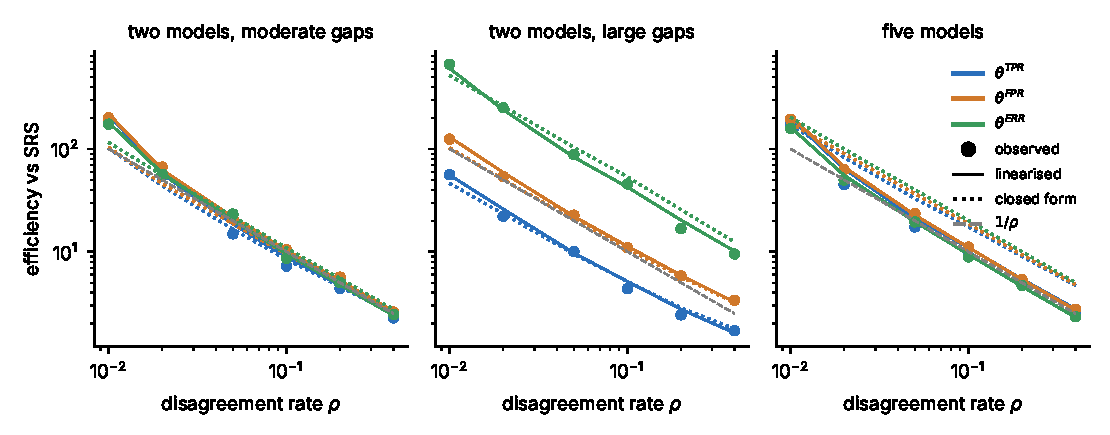
\includegraphics[width=\textwidth]{figures/fig_sim_rho.pdf}
\caption{Synthetic pools: efficiency of PATTERN relative to SRS against the disagreement rate
$\rho$ (share of the pool in the disagreement region), median over pairs for each type of estimand.
Points: Monte Carlo ($R=1000$); solid: linearised prediction LIN; dotted: closed form FORM;
grey dashed: $1/\rho$. Source: \texttt{results/theory\_check.json}.}
\label{fig:sim-rho}
\end{figure}

\paragraph{Efficiency scales as $1/\rho$.} In all three families the efficiency falls in proportion
to $1/\rho$ over a forty-fold range of $\rho$ (Figure~\ref{fig:sim-rho}). With two models and
moderate gaps, $\rho$ times the median observed efficiency is between 0.86 and 1.13 for
$\rho\ge2\%$, so the rule of thumb is accurate to about 15\%; at $\rho=1\%$ it is 1.9, because the
budget of 1000 labels is then about half the size of the disagreement region and the
finite-population correction roughly doubles the gain. LIN agrees with the observed efficiencies
throughout (median ratio per scenario between 0.88 and 1.04), with a tendency to be optimistic by a
few per cent that we attribute to the second-order terms neglected by the linearisation.

\paragraph{The closed form is accurate, and conservative, when its assumptions hold.} With two
models, the observed efficiency of the own-target Neyman design divided by FORM is between 0.90 and
1.25 for moderate gaps and $\rho\ge5\%$, and between 0.95 and 1.47 for large gaps; the LIN
predictions for the same designs give the same ratios, so the discrepancy is in the closed form and
not in the simulation. FORM is below the truth for two reasons stated in
Corollary~\ref{prop:deff}(a): it treats the agreement region as one stratum, whereas the pattern
design splits it by the common prediction ($K=0$ versus $K=M$, which have very different positive
rates), and it ignores the finite-population correction, which matters when the disagreement region
is small (at $\rho=1\%$ the ratio is 1.5 to 2.5). The large-gap family also shows the role of the
target size in Corollary~\ref{prop:deff}(c): the TPR gaps are large and the disagreements one-sided
($|a_g|=0.9$), and the gain for $\theta^{TPR}$ is only 0.45 to 0.7 times $1/\rho$, in line with
the factor $(\beta+\lambda)^{-2}$, which is about 0.4 for group 0 ($\pi_{\mathcal D}\approx
\pi_{\mathcal A}\approx0.3$) before the group factor $\Gamma$ is applied, while for the error difference, whose disagreements are nearly
deterministic within each group ($|\mu_g|=0.9$), the gain is several times $1/\rho$, as
\eqref{eq:deff-err} predicts.

\paragraph{With more models, the relevant rate is between $\rho_{\rm any}$ and the pairwise rate.} In
the five-model family the pairwise disagreement rate is about half of $\rho$, and FORM, which assumes
that each pair's disagreements are isolated, overstates the gain by a factor of about 1.9 (median
ratio of observed to FORM between 0.53 and 0.56 for $\rho\ge2\%$). The observed efficiency is instead
close to $1/\rho_{\rm any}$ ($\rho_{\rm any}$ times the median efficiency is between 0.94 and 1.03 for
$\rho\ge2\%$), the lower end of \eqref{eq:deff-sandwich}. This is expected: in this family the models
err independently inside the disagreement region, so a pair's disagreements are spread evenly over
the values of $K$. In the real pools, where models make correlated errors, the median OWN efficiency
lies inside the interval $[1/\rho_{\rm any},1/\rho]$ for every pool (Table~\ref{tab:sim-real}),
mostly in its lower half.

\subsection{Misspecified proxy}\label{sec:sim-proxy}

Proposition~\ref{prop:proxy} bounds the loss from a wrong proxy by the ratio \eqref{eq:proxy-loss}.
We took the five-model pool with $\rho=5\%$ and compared allocations computed from the default proxy,
from the true labels (oracle), from a constant proxy equal to the overall positive rate
(uninformative), from one minus the default proxy (inverted), and from an adversarial proxy that sets
$\pi_i=0.5$ where all models agree and $\pi_i=0.001$ where they do not, with proportional allocation
on the same strata as a reference.

\begin{table}[t]
\centering
\caption{Proxy misspecification (five models, $\rho=5\%$, $L=1000$, $R=1000$). Loss: weighted
variance $\sum_tw_tV_t$ relative to the oracle allocation, predicted by the linearisation (pred.) and
observed with MSEs (obs.). Eff: harmonic mean over the 30 estimands of the efficiency relative to
SRS, predicted and observed, and the smallest observed efficiency. Kant.: Kantorovich bound of
Proposition~\ref{prop:proxy}(c) evaluated with the actual allocation. Source:
\texttt{results/theory\_check.json}.}
\label{tab:sim-proxy}
\small
\begin{tabular}{lrrrrrr}
\toprule
Allocation & Loss pred. & Loss obs. & Eff pred. & Eff obs. & min Eff obs. & Kant.\\
\midrule
Default proxy & 1.00 & 1.01 & 22.0 & 20.5 & 15.4 & 1.24\\
Oracle & 1.00 & 1.00 & 21.9 & 20.6 & 17.1 & 1.07\\
Uninformative & 1.00 & 1.01 & 21.9 & 20.5 & 16.6 & 1.23\\
Inverted & 1.00 & 0.98 & 22.0 & 21.2 & 17.2 & 1.24\\
Adversarial & 1.00 & 0.98 & 21.9 & 21.0 & 15.9 & 1.21\\
Proportional & 8.48 & 7.85 & 2.6 & 2.6 & 2.1 & 56.21\\
\bottomrule
\end{tabular}
\end{table}

None of the four wrong proxies costs a measurable amount of efficiency (Table~\ref{tab:sim-proxy}):
the predicted loss is at most 0.2\%, the observed differences (between $-2.4\%$ and $+1.2\%$) are
within Monte Carlo error, and every one of the 30 estimands is estimated at least 15 times more
efficiently than under SRS. Proportional allocation on the same strata, by contrast, has eight times
the weighted variance. The explanation is Proposition~\ref{prop:influence}: the proxy enters the
anticipated stratum variances only through label rates, while the dominant feature, namely that the
comparison estimands receive almost no variance from the strata where all models agree, is fixed by
the predictions. With a constant or adversarial proxy the agreement strata are still anticipated to
have variance of order $\delta_g^2$, which is small, and the disagreement strata still have variance
of order one because $D_i$ varies within them; so all these allocations put almost the whole budget
into the disagreement strata and differ only in how it is divided among them. The Kantorovich bounds
(1.21--1.24) are valid but loose here. This robustness is specific to the structure of the problem
and should not be read as a general guarantee: Proposition~\ref{prop:proxy}(d) shows that a proxy
that misjudges a high-variance stratum can do arbitrarily badly in other stratified problems, and the
empirical comparison with the oracle allocation in Section~\ref{sec:empirical} is the relevant check
for real data.

\subsection{Summary}

The linearised design effect predicts the efficiency of the implemented design to within Monte
Carlo error on all 11 real pools and in the synthetic families (per-target median ratio 1.00,
10\%--90\% range 0.83--1.22 on the real pools). The closed form of Corollary~\ref{prop:deff} is
accurate and conservative when the strata separate a pair's agreements from its disagreements (the
own-target efficiency is 0.90 to 1.47 times the formula for $\rho\ge5\%$), and it captures the $1/\rho$ scaling and the effect of the
target size. With nine models it overstates the gain on real pools by a median factor of about two,
because the counts $K$ locate any disagreement but not that of a specific pair; the bounds
$1/\rho_{\rm any}\le\mathrm{Eff}\le1/\rho$ of \eqref{eq:deff-sandwich} describe this gap. The gain vanishes
only as the disagreement rate approaches one, as in EEG ($\rho_{\rm any}=0.73$, efficiency 1.6--1.9).
